\section{研究背景与思路}
\subsection{研究背景}
新型冠状病毒肺炎(Corona Virus Disease 2019,COVID-19),简称“新冠肺炎”,世界卫生组织命名为“2019冠状病毒病”   ,是指2019新型冠状病毒感染导致的肺炎。2019年12月截至欧洲中部夏令时间2022年6月8日,全球累计新冠肺炎确诊病例5.3亿例,累计死亡病例630万例。

秦皇岛,是河北省辖地级市,国务院批复确定的中国环渤海地区重要的港口城市,著名的滨海旅游、休闲、度假胜地,因秦始皇东巡至此派人入海求仙而得名,是中国唯一一个因皇帝帝号而得名的城市,因《浪淘沙·北戴河》而闻名遐迩,汇集了丰富的旅游资源,是驰名中外的旅游休闲胜地,山海关区是国家历史文化名城。

秦皇岛旅游业是秦皇岛的支柱产业之一,拉动了第三产业的发展,占据了秦皇岛GDP的相当比重。
新冠疫情对人民群众生命健康安全造成了严重威胁,经济停滞,物流受阻,对秦皇岛,中国乃至世界旅游业造成了巨大冲击。从长期看,冲击是暂时的,不会对我国旅游产业的基本面造成改变。中国共产党始终把人民群众生命安全和身体健康放在第一位,在党中央高度重视、科学部署下,新冠疫情得到有效控制。2020年中国GDP为101.4万亿元,比上年增长2.2\%,是全球主要经济体中唯一实现经济正增长的国家。2021年中国GDP总量达到114.4万亿元人民币,实际GDP同比增长8.1\%。

国内疫情控制局面良好的背景下,秦皇岛旅游业也逐渐回暖。但在2022年,新冠病毒变异株Omicron迅速席卷全球,输入到中国境内。2022年2月秦皇岛毗邻城市葫芦岛疫情,3月长春疫情,4月上海疫情再次对秦皇岛乃至中国旅游业造成冲击。疫情对2020,2021年秦皇岛旅游业的影响有多大?影响的趋势如何?因此,研究新冠疫情对秦皇岛旅游业的影响具有重要意义。



\subsection{研究思路}
本文通过2012-2019年秦皇岛接待游客总数构建SARIMA模型,使用SARIMA模型对2020,2021年接待游客总数,通过与实际接待游客总数进行对比,探究新冠疫情对秦皇岛2020,2021年旅游业的影响。再通过SARIMA模型得出的新冠疫情对2020,2021秦皇岛影响的数据确定两年每个月的影响因子。通过对24个影响因子进行神经网络回归,进而预测2022年每个月的影响因子,从而预测2022年旅游业的发展趋势。

具体研究思路如下:


\begin{figure}[htbp]
	\centering
	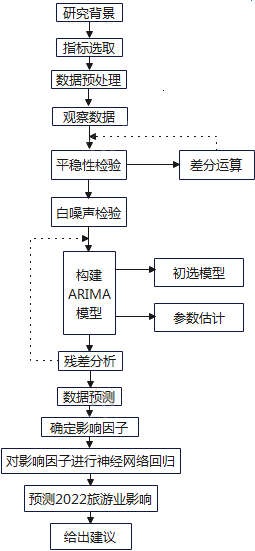
\includegraphics[scale=0.75,angle=0]{images/1.png}
	\caption{论文研究思路}
	\label{1}
\end{figure}



\section{SARIMA模型和神经网络回归模型}
	\subsection{SARIMA模型}
		\subsubsection{自回归模型(AR(p))}
		对于一个时间序列$\{\xi _t:t \in N\}$,如果对任意$t \in N$,$\{\xi_t \}$满足
		\begin{gather}
		1^{\circ} ~~~~\xi_t=\varphi_1 \xi_{t-1}+ \dots + \varphi_p \xi_{t-p} + \varepsilon_t =\sum_{i=1}^{p} \varphi_i\xi_{t-i}+\varepsilon_t 
		\\
		2^{\circ} ~~~~\forall t<s,E(\xi_t\varepsilon _s)=0
		\end{gather}
		则称$\{\xi_t\}$满足自回归模型,其中  $p>0, \varphi_{p} \neq 0,\left\{\varepsilon_{t}\right\} $ 为白噪声, 即  $E\left(\varepsilon_{t} \cdot \varepsilon_{s}\right)=0(t \neq s), E \varepsilon_{t}^{2}=\sigma_{\varepsilon}^{2}   >0, \varphi_{i}(i=1,2, \cdots, p) $ 为常数;
		$p$称为自回归模型的阶数. 自回归模型用 $ \mathrm{AR}(p)  $表示.
		
		不难看出$\{\xi_t\}$是当前的一个信号,它与前面$p$个信号有关,而$\{\varepsilon_{t} \}$是当前信号的干扰,它不会干扰到当前信号之前的信号。
		
		
		
		\subsubsection{滑动和模型((MA(q))}
		如果时间序列 $ \left\{\xi_{i}\right\}  $对任一 $ t \in \mathbf{N} $, 有
		\begin{gather}
		1^{\circ} ~~~~\xi_{t} =\varepsilon_{t}-\theta_{1} \varepsilon_{t-1}-\cdots-\theta_{q} \varepsilon_{t-q}=-\sum_{i=0}^{q} \theta_{i} \varepsilon_{t-i} 
 	\\
		2^{\circ} ~~~~ \forall  t<s  ,  E\left(\xi_{t} \cdot \varepsilon_{s}\right)=0 .
		\end{gather}
		其中,$\left(\theta_{0}=-1, \theta_{i}(i=1,2, \cdots, q)\right.  $为常数,,$ \left.\theta_{q} \neq 0\right)$ ;称 $  \left\{\xi_{t}\right\}  $满足滑动和模型,用 MA  (q)  表示上述滑动和模型,  q  称为  $\operatorname{MA}(q) $ 的阶数.
		\subsubsection{自回归滑动和模型((ARMA(p,q))}
		如果时间序列 $ \left\{\xi_{i}\right\}  $对任一 $ t \in \mathbf{N} $, 有
		\begin{gather}
		1^{\circ} ~~~~ \xi_{t}-\varphi_{1} \xi_{t-1}-\cdots-\varphi_{p} \xi_{t-p} = \varepsilon_{t}-\theta_{1} \varepsilon_{t-1}-\cdots-\theta_{q} \varepsilon_{t-q},
	\\
		2^{\circ} ~~~~ \forall  t<s  ,  E\left(\xi_{t} \cdot \varepsilon_{s}\right)=0 .
		\end{gather}
		$\text { 其中 } \varphi_{1}, \varphi_{2}, \cdots, \varphi_{p}, \theta_{1}, \theta_{2}, \cdots \theta_{q} \text { 均为常数; } \varphi_{p} \neq 0, \theta_{q} \neq 0 \text {; }$
		则 $ \left\{\xi_{t}\right\}  $称为自回归滑动和序列, 或称 $ \left\{\xi_{t}\right\} $ 满足自回归滑动和模型. 记为  $\mathrm{ARMA}(p, q),(p, q) $ 称为模型的阶数.
		不难看出 $ \operatorname{ARMA}(p, q) \text { 模型包含了 } \mathrm{AR}(p) \text { 和 } \mathrm{MA}(q)$。
		
		\subsubsection{ARIMA模型}
		ARIMA模型在ARMA的基础上引入了差分运算。首先介绍差分运算。\cite{book3}
		\\
		相距一期的两个序列使之间的减法运算称为 1阶差分运算。记 $ \nabla x_{t} $ 为  $x_{t}  $的 1 阶差分:
	$$	\nabla x_{t}=x_{t}-x_{t-1}$$
		对 1 阶差分后序列再进行一次 1 阶差分运算称为 2 阶差分。记 $ \nabla^{2} x_{t}  $为  $x_{t} $ 的 2 阶差分:
	$$	\nabla^{2} x_{t}=\nabla x_{t}-\nabla x_{t-1}$$
		依此类推, 对  p-1  阶差分后序列再进行一次 1 阶差分运算称为  p  阶差分。 记  $\nabla^{p} x_{t} $ 为 $ x_{t}  $的  p  阶差分:
	$$	\nabla^{p} x_{t}=\nabla^{p-1} x_{t}-\nabla^{p-1} x_{t-1}$$
	假设 $ \mathrm{p} , \mathrm{q} ,\mathrm{~d}  $已知,$ARIMA(p,d,q)$可以表示为:
	$$\nabla^{d} y_{t} =\varphi_{0}+\varphi_{1} \nabla^{d} y_{t-1}+\ldots+\varphi_{p}  \nabla^{d} y_{t-p}+\varepsilon-\theta_{1}  \varepsilon_{t-1}-\ldots+\theta_{q}  \varepsilon_{t-q}$$
	其中,  $\varphi $ 表示 $ AR $ 的系数,  $\varepsilon $ 表示$  MA$  的系数。
		\subsubsection{SARIMA模型}
		SARIMA模型是在ARIMA模型上的进一步扩展,SARIMA通过周期间隔上做ARIMA,可以适应季节性的时间序列,SARIMA模型可以表示为:
 $$ARIMA(p, d, q) * (P, D, Q)^s $$该式子满足乘法原则,前半部分表示非季节部分,后面表示季节部分,s表示季节性频率。
	\subsection{神经网络回归模型}
	\subsection{神经网络}
	神经网络是一种模仿动物神经元而产生的模型,可用于分类,回归等问题,模型效果良好。神经网络在理论上能够拟合任意函数,包括非线性函数,是当下最流行的数学建模方法之一。
	
	1959年两个生物科学家发现青蛙的神经元接受多个输入,输入包括青蛙的多个器官的输入,只有单输入的和到达一个阈值,才会有输出(青蛙接受的刺激比较大时才会有反应。)
	于是计算机科学家仿照生物神经元的原理和结构,提出了感知器,感知机可以表示为$$y=o(\sum_{i=0}^{n} w_{i} x_{i}+w_0),$$其中
	
$$	o(x)=\left\{\begin{array}{c}
		1 ,~~~~x>0 \\
		0, ~~~~x \leq 0
	\end{array}\right.
	$$
	\begin{figure}[h]
		\centering
		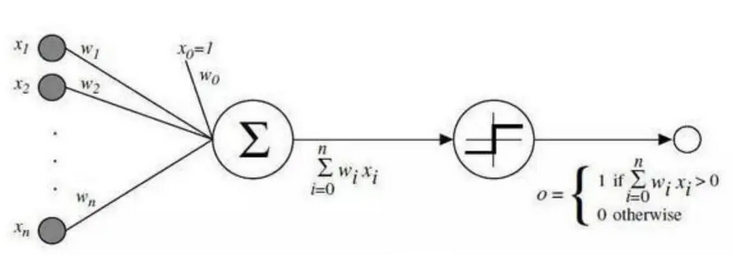
\includegraphics[scale=0.5,angle=0]{images/3.png}
		\caption{感知器}
		\label{3}
	\end{figure}
	在感知机的基础上,科学家们设置了输入层,隐藏层,输出层,并在每一层设置若干个感知机,形成了神经网络。
	\begin{figure}[h]
		\centering
		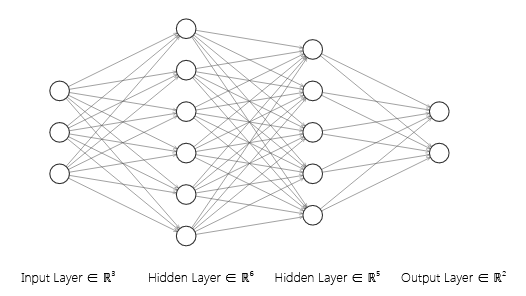
\includegraphics[scale=0.75,angle=0]{images/4.png}
		\caption{神经网络}
		\label{4}
	\end{figure}
	神经网络使用剃度下降法求解最优值,剃度下降法是一类求解函数最小值的计算机算法。假设希望求解目标函数 
	 $ f(x)=f(x_1,\dots ,x_n) $的最小值,可以从一个初始点 $ x^{(0)}=(x_1^{(0)},\dots ,x_n^{(0)}) $开始,基于学习率 $\alpha > 0$ 构建一个迭代过程:\begin{gather*}
x_1^{i+1}=x_1^{i}+\alpha \frac{\partial f}{\partial x_1}(x^{(i)})\\
 \vdots \\
x_1^{i+1}=x_1^{i}+\alpha \frac{\partial f}{\partial x_1}(x^{(i)})
\end{gather*}	 其中$x^{(i)}=(x_1^{(i),\dots,x_n^{(n)}}),i>=0$,一旦达到收敛条件的话,迭代就结束了。图\ref{5}是用剃度下降法求解$y=x^2$的最小值时迭代10次的过程,其中的点代表每次迭代后的值。
\begin{figure}[h]
\centering
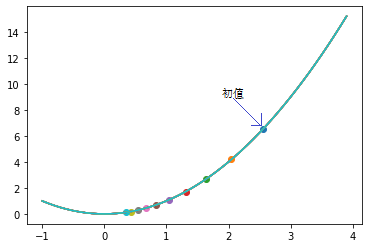
\includegraphics[scale=0.7,angle=0]{images/5.png}
\caption{剃度下降法图解}
\label{5}
\end{figure}
\subsection{LSTM}
LSTM,又称长短记忆单元,是在神经网络基础上发展形成的模型,可以提取长期序列的信息并有一定的遗忘功能。LSTM主要有三个门:忘记门,输入门,输出门。

忘记门用于过滤信息,决定了从状态中丢弃什么信息:$$f_{t}=\sigma\left(W_{f} \cdot\left[h_{t-1}, x_{t}\right]+b_{f}\right)$$忘记门会读取前一序列中的输出$h_{t-1}$和当前模型的收入$x_t$,来控制细胞状态$C_{t-1}$中的每个数字是否保留。
\begin{figure}[h]
	\centering
	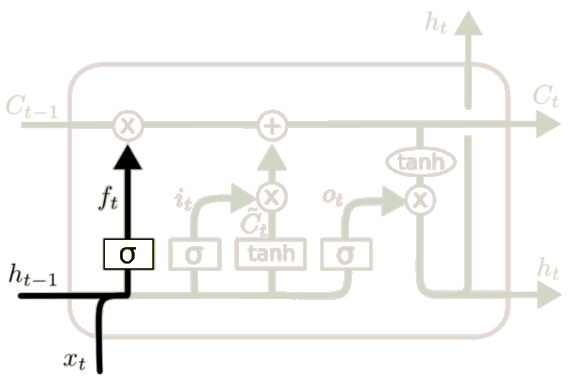
\includegraphics[scale=0.5,angle=0]{images/21.png}
	\caption{遗忘门结构}
	\label{21}
\end{figure}
其中, $ f_{t} $ 代表忘记门的输出结果, $ \sigma $ 代表激活函数,  $W_{f} $ 代表忘记门的权重,  $x_t$ 代表当前模型的输入, $ \boldsymbol{h}_{t-1} $ 代表前一个序列模型的输出, $ \boldsymbol{b}_{f} $ 代表忘记门的偏置。

输入门部分包括输入门和输入门更新。输入门公式为:
\begin{align*}
	i_{t}=\sigma\left(W_{i} \cdot\left[h_{t-1}, x_{t}\right]+b_{i}\right) \\
	C_{t}=\tanh \left(W_{C} \cdot\left[h_{t-1}, x_{t}\right]+b_{C}\right)
\end{align*}

输入门状态更新公式为:$$C_{t}=f_{t} * C_{t-1}+i_{t} * \tilde{C}_{t}$$

\begin{figure}[h]
	\centering
	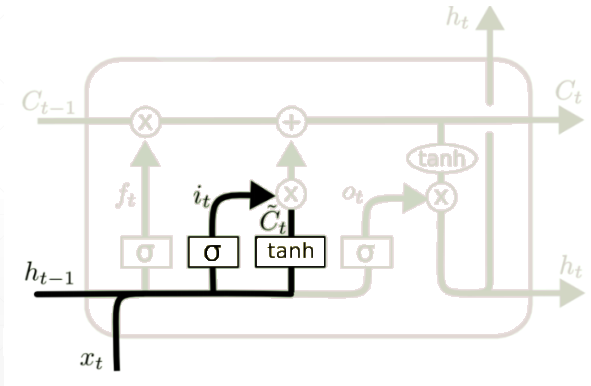
\includegraphics[scale=0.5,angle=0]{images/22.png}
	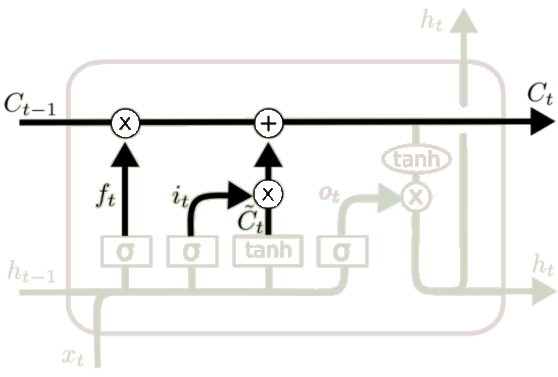
\includegraphics[scale=0.5,angle=0]{images/24.png}
	\caption{输入门和输入门更新}
	\label{21}
\end{figure}

忘记门找到了需要忘掉的信息 $ \boldsymbol{f}_{t} $ 后,再将它与旧状态相乘,丢弃确定需要丢弃的信息。然后, 将结果加上 $ i_{t} \times \tilde{C}_{t} $ 使细胞状态获得新的信息。这样就完成了细胞状态的更新。

输出门用于输出想要的部分,公式如下:
\begin{align}
	o_{t}=\sigma\left(W_{o}\left[h_{t-1}, x_{t}\right]+b_{o}\right) \\
	h_{t}=o_{t} * \tanh \left(C_{t}\right)
\end{align}

在输出门中, 通过一个激活函数层(实际使用的是 $Sigmoid$ 激活函数) 来确定哪个部分的信息将输出, 接着把细胞状态通过 $ \tanh $ 进行处理 (得到一个在 $ -1 \sim 1$  的 值 ), 并将它和$ Sigmoid $门的输出相乘,得出最终想要输出的那个部分。

\begin{figure}[h]
	\centering
	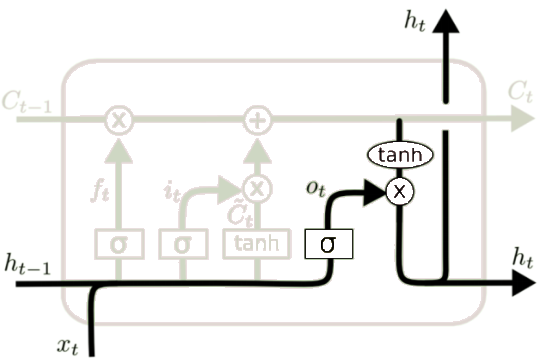
\includegraphics[scale=0.5,angle=0]{images/23.png}
	\caption{输出门}
	\label{23}
\end{figure}

\section{秦皇岛旅游接待人数的SARIMA模型}
	\subsection{指标选取及数据预处理}
		\subsubsection{指标选取}
		根据秦皇岛统计局的数据,本文初步选取了旅游收入和接待游客数量作为衡量秦皇岛旅游数据的指标,其中旅游收入包括国内收入和外汇收入,接待人数包括国内游客人数和国外游客人数。最终选择接待游客总人数作为衡量指标,即国内收入和外汇收入的和,原因如下:(1)旅行过程中旅客的所有消费都会别记录为旅游收入,相比旅游收入,接待人数具有更好的准确性。(2)秦皇岛统计局给出的旅游收入统计口径不一,缺失的数据较多。(3)根据历年数据,国外游客的数量远远少于国内游客,平均仅占0.722\%,加之国外疫情严重,来华游客大幅减少,部分缺失外国游客接待数的数据,可以将国内游客接待数近似看成总接待人数。
		\subsubsection{数据预处理}
		秦皇岛2012-2021年旅游接待人数数据具有相当一部分的缺失。本文主要采用了一下四种方法进行填充:
		
		\textbf{(1)逻辑推理}~~~~如果知道$y$年$m$月接待游客总数为$sum$,增长率为$rate$,则$y-1$年$m$月的接待游客总数$sum_{y-1}$为:$$sum_{y-1}=\frac{sum}{1+rate}$$
		
		\textbf{(2)均值填充}~~~~由于统计局的统计口径是每年2月开始统计累计值,如果一年中仅缺失前$a(a\leq 3)$个月数据的,采用平均值填充
		$$sum_i=sum_{a+1}\frac{i}{a+1},~~~~~~~i \leq a$$
		
		\textbf{(3)平均值填充}~~~~不属于第二种情况,一年中只缺失一个数据并且不是最后一个月的,使用前后两个月数据进行平均值填充:$$sum_i=\frac{sum_{i-1}+sum_{i+1}}{2}$$
		
		\textbf{(4)平均增长率填充}~~~~一年缺失数据大于3个且不满足前面三个的,假设当年缺失数据为$sum_1,sum_2,\dots,sum_a$,已知当年已知数据的增长率$rate_{a+1},rate_{a+2},\dots,rate_{12-a}$以及缺失数据上一年对应月的数据$lastsum_1,lastsum_2,\dots,lastsum_a$,则$$sum_i=lastsum_i\frac{\sum_{i=a+1}^{12-a} rate_i}{12-a}$$
	\subsection{时间序列预处理}	
	\subsubsection{平稳性检验}
	根据2012年-2021年每月秦皇岛接待游客总人数数据,绘制曲线图如下:
		\begin{figure}[H]
			\centering
			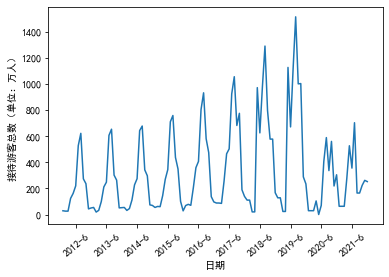
\includegraphics[scale=0.5,angle=0]{images/6.png}
			\caption{秦皇岛2012-2021接待游客总数趋势}
			\label{6}
		\end{figure}
	
	从曲线图中可以看出,2020,2021年旅游接待总人数明显下降,说明秦皇岛旅游业确实受到了疫情的冲击。根据曲线图,明显看出改序列不是一个平稳序列,长期具有上升的趋势,并且受季节周期性波动,不符合时间序列建模条件。因此对2012-1到2019-12数据进行一阶季节12步差分,即$sum_i=sum_{i+12}-sum_i$,得到的数据如图所示:
\begin{figure}[H]
	\centering
	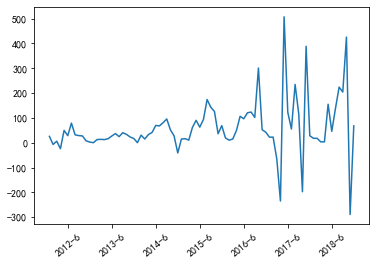
\includegraphics[scale=0.5,angle=0]{images/8.png}
	\caption{秦皇岛2012-2019接待游客总数一阶季节差分趋势图}
	\label{8}
\end{figure}
经过一阶逐步差分和一阶季节差分,数据已经消除了趋势性和周期性,下面进行数据平稳性检验。
假设原始数据$\{\xi_i\}$的$AR(p)$模型为:$$\xi_t=\varphi_1 \xi_{t-1}+ \dots + \varphi_p \xi_{t-p} + \varepsilon_t,$$则令$$\rho=\varphi_{1}+\varphi_{2}+\cdots+\varphi_{p}-1$$ 
\begin{center}$H_{0}: \rho<0  $(序列  $\xi_{t} $ 平稳) $ \leftrightarrow H_{1}: \rho=0  $(序列  $\xi_{t} $ 非平稳)  \end{center}
ADF检验统计量为:
$$\tau=\frac{\hat{\rho}}{S(\hat{\rho})}$$
式中, $ S(\hat{\rho}) $ 为参数 $ \rho $ 的样本标准差。使用EVIEW6.0软件求得ADF值及临界值如下:
\begin{figure}[htbp]
	\centering
	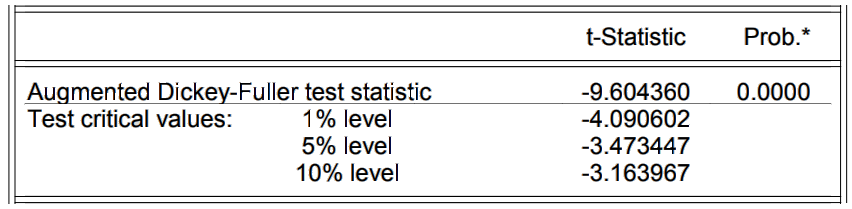
\includegraphics[scale=0.65,angle=0]{images/9.png}
	\caption{ADF平稳性检验}
	\label{9}
\end{figure}

得ADF的检验值为$-9.60$,小于1\%的临界值$-4.09$,接受原假设,认为序列平稳。
\subsubsection{白噪声检验}
对于时间序列$\{x_i\}$,任意取观察期数为n的观察序列$\left\{x_{t}, t=1,2, \cdots, n\right\}$,该样本的$k$阶非零延迟期数自相关系数为$\hat{\rho}_k$,则
\begin{align*} 
 &H_{0}  : \text{至少存在某个} \rho_{k} \neq 0, \forall m \geqslant 1, k \leqslant m \text{(序列 $ x_{i} $ 不是白噪声)} 
\leftrightarrow \\
 &H_{1}: \rho_{1}=\rho_{2}=\cdots=\rho_{m}=0, \forall m \geqslant 1  \text{(序列$x_{i} $是白噪声)}
\end{align*}
$LB$检验统计量为$$Q_{LB}= n(n+2) \sum_{k=1}^{m}\left(\frac{\hat{\rho}_{k}^{2}}{n-k}\right)$$
使用EVIEW6.0可得数据的自相关系数和偏自相关系数图:
\begin{figure}[htbp]
	\centering
	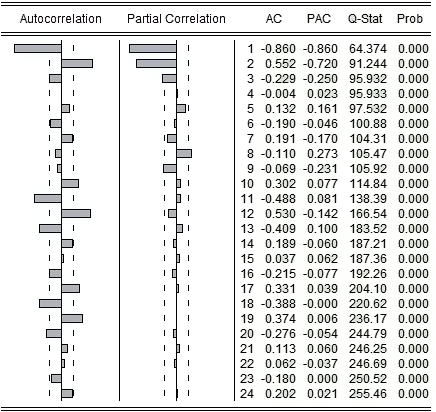
\includegraphics[scale=1,angle=0]{images/10.png}
	\caption{自相关系数和偏自相关系数图}
	\label{10}
\end{figure}

由数据结果易知,Q统计量的值均不为零,故接受原假设,即认为数据不是白噪声序列,满足建模条件。
	\subsection{模型构建}
		\subsubsection{初选模型}
		根据前面的分析,$SARIMA(p,d,q)(P,D,Q)^s$ 中 $d=0,D=1,s=12$,由于 k=12, 时序列自相关系数和偏自相关系数都不显著为0,因此考虑$ P=1,Q=1$。观察序列自相关系数和偏自相关系数图发现,自相关系数拖尾。而偏自相关系数表现为2阶截尾,$k=8,k=9$时有增大趋势,因此考虑$p=0,q=1$或$q=2$。
		因此,初选模型$SARIMA(0,0,1)(1,1,1)^{12}$,$SARIMA(0,0,2)(1,1,1)^{12}$。
		\subsubsection{参数估计}
		采用极大似然估计法对筛选出的模型进行参数估计,结果如下:
		\begin{figure}[htbp]
			\centering
			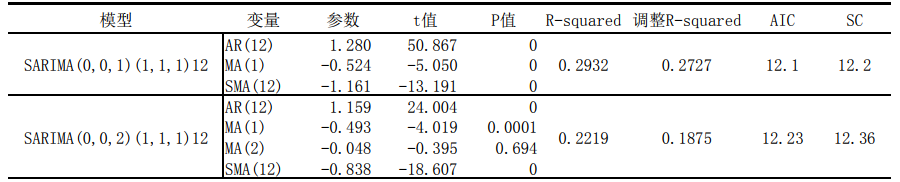
\includegraphics[scale=0.7,angle=0]{images/11.png}
			\caption{模型参数估计结果}
			\label{11}
		\end{figure}

	$SARIMA(0,0,2)(1,1,1)^{12}$没有通过显著性检验的模型,并且AIC和SC值较大,因此选择$SARIMA(0,0,1)(1,1,1)^{12}$作为最终模型。
		\subsubsection{残差分析}
		对$SARIMA(0,0,1)(1,1,1)^{12}$进行残差检验,检验结果如下:
		\begin{figure}[htbp]
			\centering
			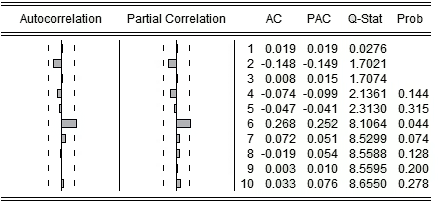
\includegraphics[scale=0.8,angle=0]{images/12.png}
			\caption{残差检验}
			\label{12}
		\end{figure}
	
	从图中可以看出,除了k=6,显著性为4.4\%,小于5\%,其他所有样本显著性检验均大于5\%,并且落在2倍标准差内,可以认为数据通过了残差检验。
	%从自相关系数和偏自相关系数图可以看出,$SARIMA(0,0,1)(1,1,1)^{12}$充分提取了数据信息,模型效果良好。
		
		
\section{基于神经网络的秦皇岛旅游接待人数的影响和预测回归模型}
	\subsection{2020、2021疫情对秦皇岛旅游业接待人数的影响程度}
	通过建立的$SARIMA(0,0,1)(1,1,1)^{12}$模型对2020,2021每个月数据进行预测,数据显示平均误差只有8.8\%,模型效果较好。
		\begin{figure}[htbp]
		\centering
		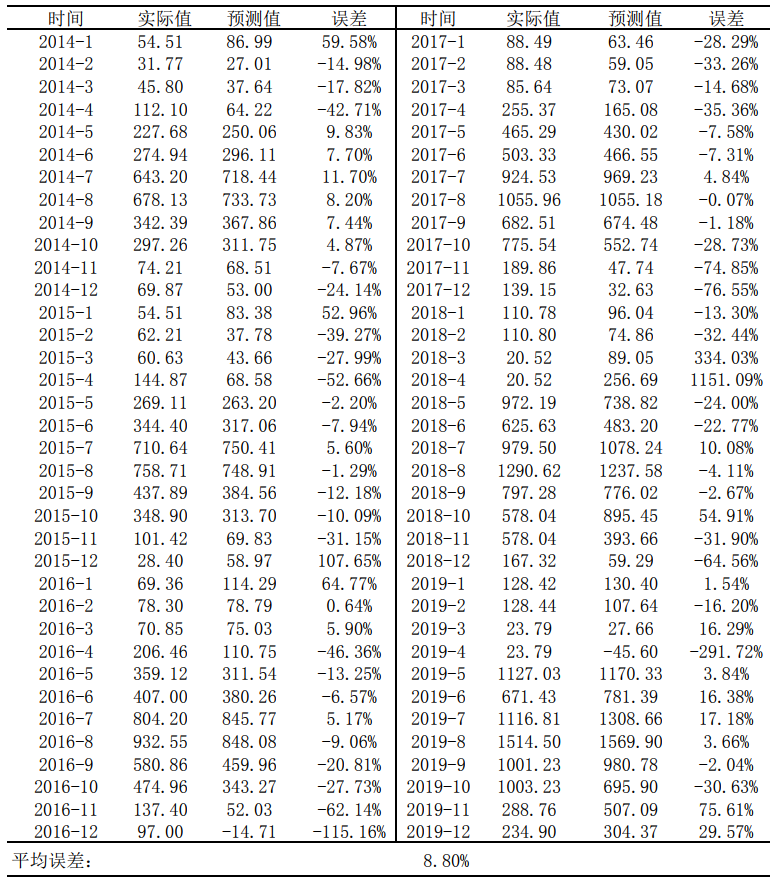
\includegraphics[scale=0.7,angle=0]{images/14.png}
		\caption{预测数据与真实数据误差}
		\label{14}
	\end{figure}

通过$SARIMA(0,0,1)(1,1,1)^{12}$模型预测秦皇岛2020年与2021年接待游客总数,同时与实际接待游客总数,可以得到疫情对接待总人数的影响。其中$\text{影响百分比}=\frac{\text{影响值}}{\text{预测数据}}$,代表了疫情时接待游客总人数减少的比例。结果如下:
		\begin{figure}[htbp]
		\centering
		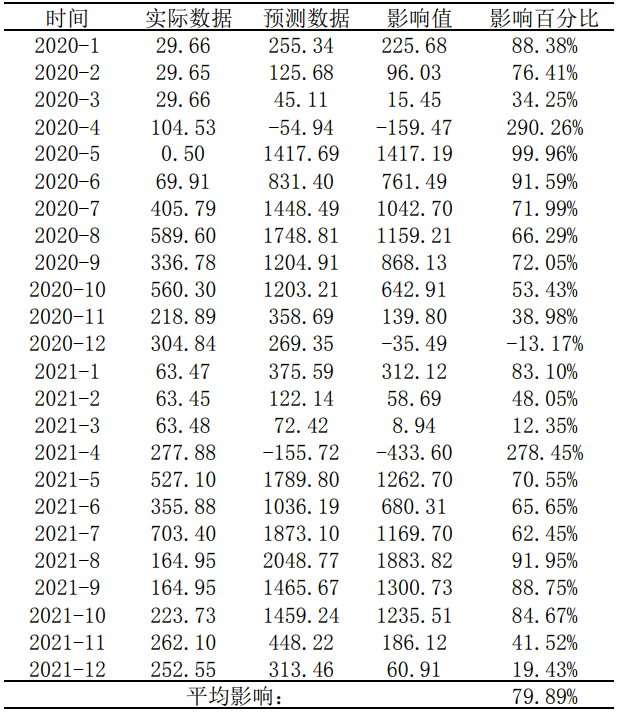
\includegraphics[scale=0.55,angle=0]{images/15.png}
		\caption{模型预测结果及其影响}
		\label{15}
	\end{figure}
	
	数据显示,受疫情影响,2020年秦皇岛旅游接待总人数减少80.87\%,2021年秦皇岛旅游接待总人数减少78.91\%,两年平均减少79.89\%。
	
	从数据来看,2002年新冠开始之初影响最大,5月份近乎夭折。但随着武汉4月全面解封,2020年疫情防控整体良好的情况下,2020年后半年疫情的影响程度逐渐减小。2021年由于德尔塔变异毒株传入中国,各地疫情零散爆发,2021年影响整体平稳偏高,到年底影响逐渐减小。
			\begin{figure}[H]
		\centering
		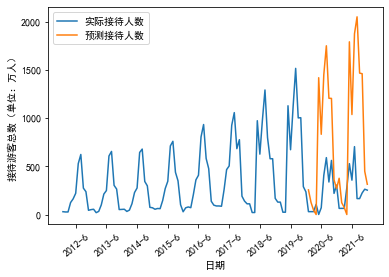
\includegraphics[scale=0.55,angle=0]{images/13.png}
		\caption{模型预测结果及其影响}
		\label{13}
	\end{figure}

	
	\subsection{预测2022年疫情对秦皇岛旅游业接待人数影响程度}
		\subsubsection{基于lstm神经网络构建回归预测模型}
		为了能够对2022年疫情影响旅游业情况进行预测,选取2012年与2019年真实的数据作为数据集训练LSTM神经网络,其中2012年-2018年为训练集,2019年为测试集。数据集具体划分如下:	
			\begin{figure}[h]
			\centering
			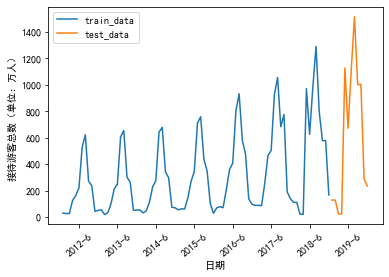
\includegraphics[scale=0.6,angle=0]{images/16.png}
			\caption{数据集划分}
			\label{16}
		\end{figure}
	
	其中参数n为24,即认定当前一个月的数据主要受过去24个月数据影响。搭建LSTM神经网络进行训练,训练次数为2500次,均方差随训练次数的变化如下图所示:\begin{figure}[h]
		\centering
		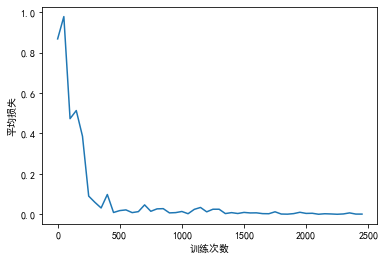
\includegraphics[scale=0.6,angle=0]{images/17.png}
		\caption{损失值变化}
		\label{17}
	\end{figure}

损失值随着训练次数增多逐渐下降并波动,最终趋向于0,说明模型在训练集上拟合效果良好。使用模型在测试集上进行训练,模型回归效果如下:\begin{figure}[H]
	\centering
	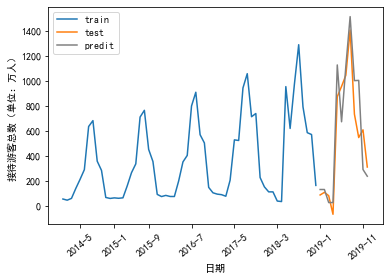
\includegraphics[scale=0.55,angle=0]{images/18.png}
	\caption{模型在测试集上的表现}
	\label{18}
\end{figure}

可以看出,在测试集上,实际曲线与预测曲线基本重合,模型在测试集上回归效果良好。
		\subsubsection{基于回归模型对2022年影响程度进行预测}
		基于上面建立的LSTM模型,使用2020年,2021年的数据,即疫情后24个月的数据,逐步预测2022年12个月秦皇岛接待游客的总人数,预测结果图示如下:\begin{figure}[h]
			\centering
			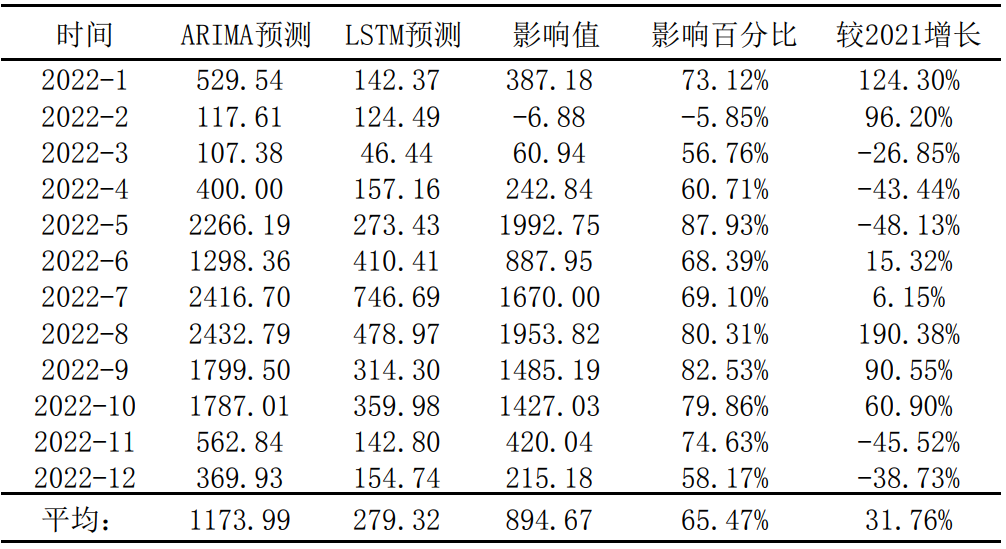
\includegraphics[scale=0.5,angle=0]{images/20.png}
			\caption{2022年预测结果}
			\label{20}
		\end{figure}
	
	从数据可以看出,疫情对秦皇岛2022年旅游业的冲击依然很大,相比疫情前,2022年秦皇岛接待游客总数相比疫情前减少65.47\%,但是比2021年减少14.42\%,说明疫情对秦皇岛的旅游业影响变小,秦皇岛旅游业正逐步变暖。2022年秦皇岛接待游客总量预计比2021年增长31.76\%,符合刚才的判断。
	\clearpage
	
		\begin{figure}[h]
			\centering
			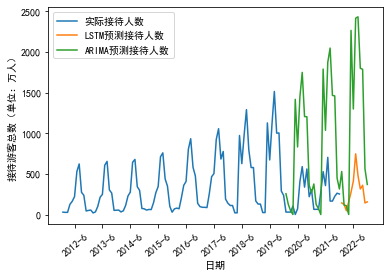
\includegraphics[scale=0.55,angle=0]{images/19.png}
			\caption{2022年预测结果对比}
			\label{19}
		\end{figure}
		绘制曲线图,任然可以得出相似的结论,从曲线图中可以发现,疫情对秦皇岛2022年旅游业的冲击相对疫情前依然很大,但相比2020与2021年,曲线呈上升趋势,说明疫情对秦皇岛的旅游业影响变小,秦皇岛旅游业正逐步变暖。
		
		
		
\section{主要结论和存在问题}
\subsection{主要结论}
根据以上分析,主要得出以下结论:

\textbf{(1)}受疫情影响,2020年秦皇岛旅游接待总人数减少80.87\%,2021年秦皇岛旅游接待总人数减少78.91\%,两年平均减少79.89\%。\textbf{(2)}预计疫情对秦皇岛2022年旅游业的冲击依然很大,相比疫情前减少65.47\%。\textbf{(3)}相比2020与2021年,疫情对秦皇岛的旅游业影响变小,秦皇岛旅游业相比2020,2021呈上升趋势,预计比2021年增长31.76\%。



\subsection{存在问题}
\textbf{(1)数据缺失}~~~~
搜集数据时发现缺失了一部分数据,由于数据的缺失,导致模型的预测精确度下降,预测结果出现了少量负值。由于缺失2022年的旅游数据,因此无法对未来时段秦皇岛的旅游业发展做出更准确的预测。

\textbf{(2)Omicron的影响}~~~~
2022年新冠病毒变异株Omicron输入中国境内,2月秦皇岛毗邻城市葫芦岛疫情,3月长春疫情,4月上海疫情再次对秦皇岛造成了冲击。由于缺失2022年的秦皇岛旅游数据,无法将Omicron的影响考虑到模型中。

